 %!TEX TS-program = xelatex
\documentclass[]{article}
\usepackage{hyperref}
\usepackage{listings}
\usepackage{cite}
\usepackage[utf8]{inputenc}
\usepackage{longtable}
\usepackage{tabularx}
\usepackage{graphicx}
\graphicspath{{./}}
\usepackage[margin=1in]{geometry}
\usepackage{xcolor}
\usepackage{tikz}
\usepackage{svg}
\usepackage[none]{hyphenat}
\usepackage{parskip}
\usepackage{multicol}
\usepackage{enumerate}
\usepackage{scrextend}
\usepackage{fancyhdr}
\usepackage{centernot}
\usepackage{amsthm, amssymb, amsmath, verbatim}
\usepackage{mathtools}
\usepackage{xifthen}
\usepackage{ifthen}
\usepackage[most,listings]{tcolorbox}
\usepackage{lmodern}
\usepackage{mathrsfs}
\usetikzlibrary{math}
\usetikzlibrary{backgrounds}
\usetikzlibrary{patterns,calc}
\usepackage{subcaption}
\usepackage{csvsimple, booktabs}
\usepackage{filecontents}
\usepackage{authblk}

\usetikzlibrary{arrows.meta,decorations.pathmorphing,backgrounds,positioning,fit,petri}

\svgpath{{./}}
\hypersetup{breaklinks=true}
\urlstyle{same}
\def\NavyBlue{\color[RGB]{24, 43, 73}} % Pantone 2767 [CMYK]{100, 86, 42, 42} [Hex]{#182B49}
\def\Color2{\color[RGB]{33, 93, 118}}
\def\Color3{\color[RGB]{231, 223, 200}}
\def\Color4{\color[RGB]{231, 190, 66}}
\def\Gold{\color[RGB]{198, 146, 20}} % Pantone 1245 [CMYK]{6, 35, 99, 18} [Hex]{#C69214}

\title{\textbf{Dynamics and Inequalities in Digital Social Networks: A Computational and Sociological Review}}
\author{Pengjia Cui \thanks{pcui@ucsd.edu}}
\affil{Computational Social Science \\ University of California San Diego}

\date{}

\begin{document}
	\begin{sloppypar}
	\maketitle
	\begin{abstract}
	Digital networks have profoundly transformed the ways in which individuals interact, exchange information, and establish connections, leading to the emergence of phenomena such as virality, misinformation cascades, and online polarization. This review conducts a thorough examination of the micro-macro linkages within digital social networks, analyzing how individual actions like liking, sharing, and commenting coalesce into broader systemic patterns and how these interactions are influenced by algorithmic mediation. Utilizing a multidisciplinary literature base, this study explores the interaction among user behaviors, network structures, and platform algorithms that intensify biases, strengthen homophily, and foster echo chambers. We delve into crucial dynamics including the scalability's impact on weak tie propagation, the amplification effects on influencers, and the rise of digital inequalities, employing both theoretical and empirical approaches. By synthesizing insights from sociology, network theory, and computational social science, this paper underscores the necessity for novel frameworks that integrate algorithmic processes into established micro-macro models. The conclusion presents practical strategies aimed at promoting fairer digital networks through decentralized architectures, algorithmic fairness, and improved digital inclusion, tackling significant challenges such as polarization and misinformation within networked societies. \\
		
		\noindent\textbf{Keywords: }Digital Social Networks, Micro-Macro Linkages, Algorithmic Mediation, Information Diffusion, Echo Chambers, Filter Bubbles, Digital Inequality, Network Dynamics, Polarization, Misinformation Cascades
	\end{abstract}
	
	
	

The study of social networks spans sociology, communication studies, and computational sciences, analyzing human interactions across digital and traditional contexts. Digital platforms like Facebook, Twitter, and LinkedIn have transformed how individuals connect, disseminate information, and influence collective behavior, prompting a need to reassess social ties and structural patterns in these environments.

This research highlights critical aspects such as network dynamics and digital inequalities, exploring how digital platforms reshape information flow and social interactions. Advances in computational tools, such as UCINET and Gephi, enable sophisticated analyses of these dynamics, offering insights into phenomena like echo chambers and misinformation propagation.

The paper progresses by integrating social network theories with contemporary digital practices, followed by a detailed bibliometric analysis and exploration of key academic questions around information dynamics and structural linkages in digital spaces. It concludes with actionable strategies for creating equitable digital environments, addressing challenges like polarization and misinformation. This streamlined approach not only enriches academic discussions but also guides practical applications for managing digital interactions.


\section{Under Digital Context}\label{Under Digital Context}

\subsection*{Tie Strength and Homophily}

Traditional and digital networks differ markedly in the dynamics of tie strength and homophily, which significantly influence the formation, maintenance, and evolution of relationships. In traditional networks, the strength of ties---the closeness or intensity of relationships---is often shaped by physical proximity, shared social contexts, and frequent face-to-face interactions. Granovetter's seminal study on ``The Strength of Weak Ties'' \cite{granovetter_strength_1973} underscores the pivotal role of weak ties, such as acquaintances, in bridging disparate network clusters and enabling the flow of novel information. However, maintaining these weak ties in traditional settings typically requires occasional in-person engagements, which may restrict their breadth and frequency.

Conversely, digital networks dramatically reduce the effort needed to establish and maintain weak ties. Platforms such as LinkedIn and Twitter allow individuals to form global connections effortlessly, with minimal commitment. These weak ties are especially effective in digital contexts for disseminating information widely, due to the scalability and ease of online interactions. Bakshy et al. \cite{bakshy_everyones_2011} found that weak ties predominate in the diffusion of viral content on social media, significantly amplifying their impact compared to traditional environments.

Moreover, homophily—the tendency of individuals to associate with similar others—manifests differently across network types. In traditional settings, homophily typically emerges from shared physical environments, like neighborhoods or workplaces, which inherently limit the diversity of connections and reinforce social and cultural homogeneity. McPherson et al. \cite{ WOS:000170748100017} have provided comprehensive insights into how homophily structures social networks and sustains social boundaries and inequalities.

In digital settings, while geographic boundaries become irrelevant, algorithmic recommendation systems intensify homophily in novel ways. These systems often recommend connections, groups, or content that align with users' existing preferences, which fosters the creation of ``echo chambers'' or ``filter bubbles'' \cite{pariser_filter_2011}, potentially exacerbating societal polarization. For instance, research indicates that Facebook’s algorithm enhances homophily by promoting links between users with similar demographic or behavioral characteristics \cite{lazer_rise_2015}.

Despite these challenges, digital platforms also hold the potential to disrupt traditional patterns of homophily by facilitating broader interactions across diverse communities. Platforms like Reddit and Twitter, for example, offer exposure to a range of viewpoints through public discussions and hashtags, though the degree to which this exposure leads to meaningful cross-group engagement is still under investigation.


\section{Bibliometric Analysis}\label{Bibliometric Analysis}

Bibliometrics is a multidisciplinary field that applies quantitative methods, particularly mathematical and statistical approaches, to the systematic analysis of knowledge sources. Bibliometric analysis allows us to uncover research trends, identify influential works, and map the intellectual structure of a field. The term "Bibliometrics" was formally introduced in 1969 by the British scientist Allen Richard, replacing the earlier designation "statistical bibliography." This terminology shift signaled the formal establishment of bibliometrics as a distinct field of study\cite{ WOS:A1969F015300009}. We aim to develop a more comprehensive understanding of the digital networks through bibliometric analysis. In this section, we employ \textbf{VOSviewer} \cite{WOS:000278695500019}, \textbf{CiteSpace} \cite{doi:10.1073/pnas.0307513100}, and \textbf{Gephi} \cite{ICWSM09154} for bibliometric analysis and visualization, alongside \textbf{NetworkX} \cite{SciPyProceedings_11} for advanced network analysis. These tools collectively enable a comprehensive exploration of network structures, research trends, and collaboration patterns. 

\subsection*{Data Preparation and Methods}

The analysis was performed using the Web of Science Core Collection database, which includes the following entitlements: 
WOS.IC (1993–2024), WOS.CCR (1985–2024), WOS.SCI (1900–2024), WOS.AHCI (1975–2024), WOS.BHCI (2005–2024), WOS.BSCI (2005–2024), WOS.ESCI (2005–2024), WOS.ISTP (1990–2024), WOS.SSCI (1900–2024), and WOS.ISSHP (1990–2024). 

The literature data used in this study were downloaded from the Science Citation Index Expanded (SCIE) and the Social Science Citation Index (SSCI) databases in Web of Science. SCIE and SSCI are among the most frequently used databases for bibliometric analysis \cite{ WOS:000375954300052}. These databases are widely recognized for their comprehensive coverage of scientific and authoritative publications. Furthermore, SCIE and SSCI provide citation information, keywords, and references, making them valuable resources for bibliometric studies which is necessary to the citation analysis implemented in later sections. 

This bibliometric analysis focuses on scholarly works indexed in the Web of Science Core Collection, spanning categories such as Multidisciplinary Sciences, Sociology, Social Sciences Interdisciplinary, Social Sciences Mathematical Methods, and Communication. By examining 1,859 publications, we aim to map the intellectual landscape, identify research trends, and uncover collaboration patterns in the field of social network studies.

The query in Appendix \ref{app:query} was executed on November 21, 2024, yielding a total of 1,859 results. The query result can be accessed through the following link: 

{\ttfamily\NavyBlue
		https://www.webofscience.com/wos/woscc/summary/ \\ d76d6d1f-6020-42cf-91b6-c24a7c6a6c0f-0129f5096b/ times-cited-descending/1
}

\begin{table}[htbp]
	\centering
	\caption{\label{table:Table.1}Document Type}
	\begin{tabular}{lrr}
		\toprule
		Type & Count & Percent \\
		\midrule
		Article & 1813 & 97.5 \\
		Review Article & 33 & 1.8 \\
		Early Access & 26 & 1.4 \\
		Proceeding Paper & 24 & 1.3 \\
		Book Chapters & 16 & 0.9 \\
		Editorial Material & 7 & 0.4 \\
		Correction & 2 & 0.1 \\
		News Item & 2 & 0.1 \\
		Retracted Publication & 2 & 0.1 \\
		Letter & 1 & 0.1 \\
		Meeting Abstract & 1 & 0.1 \\
		\bottomrule
	\end{tabular}
\end{table}

Table \ref{table:Table.1} presents the distribution of document types retrieved from the Web of Science on November 21, 2024, using the specified query. Out of 1,859 results, articles accounted for the vast majority (97.5\%), underscoring the prominence of peer-reviewed articles in disseminating research findings. This dominance is due to the nature of sociological research, which primarily produces theoretical frameworks or empirical studies that are best disseminated through academic journals.  

\subsection*{The Highly Cited Publications in Digital Social Networks}

To identify the most influential publications in the field of social networks, we selected the top 15 papers with the highest citations. Table \ref{table:Table.3} presents these highly cited works, including their titles, publication years, and citation counts. The citation numbers reflect the profound impact these papers have had on the academic community.

\begin{table}[htbp]
	\centering
	\caption{Top 15 Highest Cited Publications}
	\label{table:Table.3}
	\resizebox{\linewidth}{!}{\begin{tabular}{p{0.85\linewidth}|c|c}
			\toprule
			Title & Year & Citations \\
			\midrule
			Birds of a feather: Homophily in social networks & 2001 & 10923 \\
			The network structure of social capital & 2000 & 1965 \\
			Experimental evidence of massive-scale emotional contagion through social networks & 2014 & 1709 \\
			The Spread of Behavior in an Online Social Network Experiment & 2010 & 1650 \\
			Hierarchical structure and the prediction of missing links in networks & 2008 & 1434 \\
			A 61-million-person experiment in social influence and political mobilization & 2012 & 1415 \\
			Introduction to stochastic actor-based models for network dynamics & 2010 & 1307 \\
			Networks and epidemic models & 2005 & 1215 \\
			Structure and tie strengths in mobile communication networks & 2007 & 1180 \\
			Resources and relationships: Social networks and mobility in the workplace & 1997 & 1145 \\
			Inferring friendship network structure by using mobile phone data & 2009 & 1113 \\
			Quantifying social group evolution & 2007 & 1082 \\
			Social networks and health & 2008 & 1029 \\
			Filter Bubbles, Echo Chambers, and Online News Consumption & 2016 & 918 \\
			Comparing Brain Networks of Different Size and Connectivity Density Using Graph Theory & 2010 & 861 \\
			\bottomrule
	\end{tabular}}
\end{table}

Among these, two papers were published between 1991 and 2000, six papers between 2001 and 2010, and seven papers after 2010. This distribution indicates a growing interest in social networks, particularly in the past two decades. The average number of citations across these publications is 2,457, highlighting their significant influence.

Additionally, many of these publications focus on fundamental theories and methodologies, such as homophily in social networks, the structure of social capital, and the dynamics of network interactions. Notable works, such as "Birds of a Feather: Homophily in Social Networks"\cite{ WOS:000170748100017}, stand out with 10,923 citations, underscoring its foundational role in the field. Similarly, Burt’s work\cite{ WOS:000166194000008} on the network structure of social capital ranks second with 1,965 citations, reflecting its widespread application in network studies.

The prevalence of co-authored publications in this list highlights the importance of collaboration in producing impactful research. While the majority of these works are theoretical, several explore experimental and applied aspects of network science, such as large-scale social experiments and the analysis of online behavior.

\subsection*{Annual Trends of Publication}

The publication trend over time is illustrated in Figure \ref{fig:Fig.1}. Papers in this domain first appeared in the 1980s, with early works like those by \cite{ WOS:A1982NG01900001, WOS:A1982NM27900003, WOS:A1983QK14400006}, marking the foundational period of social network research. During this early phase (1982–2000), the field exhibited limited growth, likely reflecting its nascent state. Publications remained sparse due to technological constraints, limited data availability, and a relatively small research community focusing on network-related phenomena.

\begin{figure}[htbp]
	\caption{\label{fig:Fig.1}Publication Trend from 1982 to 2024}
	\includegraphics[width = 0.5\linewidth]{Cumulative_Pub_Year.png}
	\includegraphics[width = 0.5\linewidth]{Pub_Year.png}
\end{figure}

From 2000 to 2009, a gradual increase in publications can be observed. This growth coincides with the rise of digital communication technologies and early social networking platforms such as Friendster and MySpace. During this period, some network researchers started to focus on digital networks\cite{ WOS:000269632400036, WOS:000274745000002}. The availability of digital interaction data and advancements in computational tools enabled researchers to explore phenomena such as tie formation, network dynamics, and information diffusion with greater precision. Moreover, interdisciplinary collaboration between sociology, mathematics, and computer science catalyzed the field's development during this period.

The most dramatic growth occurred between 2009 and 2017, as evidenced by the sharp rise in publication records in Figure \ref{fig:Fig.1}. This surge coincides with the global adoption of large-scale online platforms such as Facebook, Twitter, and LinkedIn, which provided unprecedented opportunities for empirical studies \cite{WOS:000209041300003, WOS:000337300100030}. Notably, this period marked the publication of the seminal paper that established the foundation for computational social science \cite{doi:10.1126/science.1167742}. Researchers utilized these platforms to explore critical topics like algorithmic interventions, echo chambers, and misinformation propagation. Moreover, the rapid advancement and adoption of machine learning and big data analytics significantly enhanced the ability to analyze social networks at scale, fueling the expansion of this field.

From 2018 onward, the publication trend started increase steadily, maintaining a consistently high level of activity. This reflects the maturation of the field, where foundational concepts are well-established, and research is increasingly specialized. For example, studies have shifted toward addressing niche topics such as digital inequality, algorithmic bias, and the ethics of AI-driven networks. Moreover, challenges like restricted access to proprietary datasets\cite{ WOS:000352789600005} and privacy concerns have likely tempered the growth rate\cite{ WOS:000334339000015}.

\subsection*{The Distribution of Journals on Digital Social Networks}

Based on data from the Web of Science, out of all 1,859 publications, 13\% were published in \textit{PLOS ONE}, a journal under the open-access publisher \textbf{PLoS}. Ranking second is \textit{SOCIAL NETWORKS}, published by \textbf{Elsevier}, which accounts for 12.4\% of the total publications. In third place, with a proportion of 8.6\%, is \textit{SCIENTIFIC REPORTS}, a journal published by \textbf{Springer Nature}. The top 10 journals contributing to the field are presented in Table \ref{table:Table2}. These journals collectively represent diverse domains, ranging from general multidisciplinary science to highly focused computational and social network research. This distribution emphasizes the interdisciplinary nature of digital social networks, where insights are drawn from sociology, computer science, and applied mathematics.
	
	\begin{table}[htbp]
		\centering
		\caption{\label{table:Table2}Publicated Journals Distribution}
		\resizebox{\linewidth}{!}{\begin{tabular}{lrr}
				\toprule
				Publication Title & Count & Percent \\
				\midrule
				PLOS ONE & 242 & 13.0 \\
				\hline
				SOCIAL NETWORKS & 230 & 12.4 \\
				\hline
				SCIENTIFIC REPORTS & 160 & 8.6 \\
				\hline
				PROCEEDINGS OF THE NATIONAL ACADEMY OF SCIENCES OF THE UNITED STATES OF AMERICA & 78 & 4.2 \\
				\hline
				INFORMATION COMMUNICATION SOCIETY & 59 & 3.2 \\
				\hline
				COMPLEXITY & 57 & 3.1 \\
				\hline
				EPJ DATA SCIENCE & 40 & 2.2 \\
				\hline
				SOCIAL SCIENCE COMPUTER REVIEW & 33 & 1.8 \\
				\hline
				JASSS THE JOURNAL OF ARTIFICIAL SOCIETIES AND SOCIAL SIMULATION & 33 & 1.8 \\
				\hline
				COMPUTATIONAL AND MATHEMATICAL ORGANIZATION THEORY & 28 & 1.5 \\
				\bottomrule
		\end{tabular}}
	\end{table}

The prominence of \textit{PLOS ONE} in the publication landscape reflects the increasing value of open-access platforms in disseminating digital social network research. As a multidisciplinary journal, \textit{PLOS ONE} attracts studies that bridge sociology, computational methods, and applied network theory, making it a vital hub for interdisciplinary research. The open-access nature of the journal ensures that findings are accessible to a global audience, reinforcing the importance of equitable knowledge dissemination.

The strong representation of \textit{SOCIAL NETWORKS} and \textit{SCIENTIFIC REPORTS} highlights the coexistence of highly specialized and broad-spectrum journals in advancing this field. \textit{SOCIAL NETWORKS} stands out for its dedicated focus on theoretical and applied aspects of network analysis, appealing to researchers deeply embedded in this discipline. In contrast, \textit{SCIENTIFIC REPORTS} broadens the scope by publishing work that situates network research within a multidisciplinary framework, attracting contributions that span physical, social, and computational sciences.

The presence of journals such as \textit{EPJ DATA SCIENCE} and \textit{COMPUTATIONAL AND MATHEMATICAL ORGANIZATION THEORY} signals a growing emphasis on computational approaches and algorithmic methods in network studies. These venues cater to researchers exploring innovative methodologies, such as machine learning, big data analytics, and simulation techniques, to address complex questions about network dynamics and structure. Their inclusion in the top journals reflects the field's ongoing shift toward data-driven and computationally intensive research paradigms.

The diversity of the top journals illustrates the inherently interdisciplinary nature of digital social network research. Contributions to these journals often combine theoretical insights from sociology with computational tools from computer science and statistical modeling techniques from applied mathematics. This cross-disciplinary collaboration underscores the field's strength in addressing multifaceted social phenomena through innovative methodological frameworks.

\subsection*{Affiliations}

A detailed analysis of affiliations from the dataset reveals significant contributions from leading institutions globally, as illustrated in Figure \ref{fig:Fig.2}. The University of California (UC) system emerges as a prominent contributor, accounting for 6.445\% of all publications. Within the UC system, institutions like UC San Diego and UC Irvine stand out, highlighting their strong presence in the field of digital social network research. These UC system departments have a strong tradition of interdisciplinary research. By combining sociology, computer science, and political science, they create a fertile ground for digital network research that transcends traditional academic boundaries.

\begin{figure}[htbp]
	\centering
	\caption{\label{fig:Fig.2}Affiliation and Department Distribution}
	\includegraphics[width = \linewidth]{Affiliation_Combined.png}
\end{figure}

Other top contributors include globally renowned universities such as the University of Oxford (2.846\%), Harvard University (2.685\%), and the Massachusetts Institute of Technology (MIT, 2.202\%). These institutions underscore the centrality of their academic efforts in advancing digital network research. The University of Oxford and Harvard University's strong showing can be linked to their focus on theory-building and methodological innovation. Oxford's Mathematical, Physical, and Life Sciences Division and often contributes to computational and algorithmic aspects of network science, while its Social Sciences Division and Oxford Internet Institute (OII) focuses on applications in sociology and policy-making. Similarly, Harvard's interdisciplinary focus, particularly through centers like the Berkman Klein Center for Internet \& Society, advances the understanding of digital network phenomena such as information diffusion and power dynamics.

At the departmental level, UC San Diego's Division of Social Sciences (0.967\%) and Department of Political Science (0.806\%) emerge as leaders, alongside Yale University's Graduate School of Arts and Sciences (1.074\%) and Stanford University's School of Humanities and Sciences (0.806\%). These departments not only contribute to foundational research but also provide diverse perspectives across interdisciplinary boundaries. The data also highlights the contributions of emerging hubs like the University of Groningen and Ohio State University. 

\subsection*{Citation Network}

We first present the overall citation network of the dataset in Figure \ref{fig:Fig.4}. The size of the nodes represents the citation counts for each article, while the color indicates the publication year, with blue denoting older articles and gold representing newer ones. Then we computed the fundamental properties of the overall citation network, as summarized alongside the visualization. 

\subsubsection*{General Structure}

The overall citation network consists of 1,859 nodes and 3,636 edges, representing the extensive academic landscape of digital network research. With a low density of 0.0021, the network reflects the highly selective nature of academic citations, where only a subset of publications forms the central backbone of the field, while a significant number remain peripheral or disconnected.

\begin{figure}[htbp]
	\centering
	\caption{\label{fig:Fig.4}Overall Citation Network and Properties}
	\begin{minipage}[b]{0.45\linewidth}
		\centering
		\includegraphics[width=\linewidth]{keywords_overall}
		\caption*{(a) Citation Network Visualization}
	\end{minipage}%
	\hfill
	\begin{minipage}[b]{0.42\linewidth}
		\centering
		\vspace{-1em} % Adjust this value to align properly
		\resizebox{\linewidth}{!}{%
			\begin{tabular}{lr}
				\toprule
				\textbf{Metric} & \textbf{Value} \\
				\midrule
				Number of nodes & 1859 \\
				Number of edges & 3636 \\
				Average degree & 3.91 \\
				Density & 0.0021 \\
				Is directed & False \\
				Maximum degree & 425 \\
				Minimum degree & 0 \\
				Average clustering coefficient & 0.1381 \\
				Number of triangles & 2236 \\
				Max degree centrality & 0.2287 \\
				Max betweenness centrality & 0.2984 \\
				Max closeness centrality & 0.3388 \\
				Largest connected component size & 1293 \\
				Degree assortativity coefficient & -0.1015 \\
				Number of connected components & 524 \\
				\bottomrule
			\end{tabular}
		}
		\caption*{(b) Citation Network Properties}
	\end{minipage}
\end{figure}

At its core, the network is dominated by a single large connected component containing 1,293 nodes, representing the intellectual core of the field. This component accounts for the majority of influential and highly cited works, serving as the foundation for theoretical and methodological advancements. By contrast, the network's periphery consists of 524 smaller components, with the second-largest containing only four nodes. These smaller components likely correspond to niche areas or emerging topics that have yet to integrate fully into the broader academic discourse. To better understand the field's evolution and intellectual contributions, subsequent analyses will focus on the largest connected component.

The average degree of 3.91 indicates that most publications selectively engage with a few other works, a characteristic of focused citation practices. However, the network's centralization, marked by a maximum degree of 425, underscores the disproportionate influence of a few seminal works. These highly cited publications act as hubs, connecting diverse research areas and serving as cornerstones of the field's intellectual structure.

The negative degree assortativity coefficient (-0.1015) reveals a hierarchical organization, where highly cited works tend to connect with less-cited ones. This structure reflects a common pattern in citation networks, where foundational studies attract citations from newer or less established research, further reinforcing their centrality and shaping the field's direction.

Clustering dynamics also provide insight into the network's structure. The overall average clustering coefficient of 0.1381 suggests moderate local connectivity, with small clusters forming around specific subfields or methodologies. However, the low clustering value for the entire network highlights a lack of strong interconnections across these clusters, emphasizing the fragmented nature of the field's periphery. In contrast, the largest connected component demonstrates higher clustering (0.1986) and increased density (0.0043), signaling a more cohesive and interconnected intellectual core. The presence of 2,236 triangles within this component reflects the robust interlinkages among its key publications.

The network's dual structure, comprising a tightly integrated core and a fragmented periphery, reflects the evolutionary dynamics of an interdisciplinary field like digital network research. The core serves as the driving force for theoretical consolidation and methodological innovation, while the periphery captures the exploratory and emerging areas that may influence future directions. This interplay between the core and periphery underscores the dynamic and evolving nature of the field, highlighting the importance of both established works and novel contributions in shaping the landscape of digital network studies.

\subsubsection*{The Largest Connected Component}

The largest connected component of the citation network provides a comprehensive view of the core structure within this field of research as illustrated in Figure \ref{fig:Fig.9} using Yifan Hu layout\cite{hu_visualizing_2015}. Comprising 1,293 nodes and 3,592 edges, it represents the most interconnected cluster of publications, highlighting the works that are pivotal to the intellectual development of the domain. The average degree of 5.56 suggests that each publication is connected to several others, balancing both depth and breadth in academic discourse.

\begin{figure}[htbp]
	\centering
	\caption{\label{fig:Fig.9}Largest Connected Component and Properties}
	\begin{minipage}[b]{0.45\linewidth}
		\centering
		\includegraphics[width=\linewidth]{largest_component}
		\caption*{(a) Largest Connected Component Visualization}
	\end{minipage}%
	\hfill
	\begin{minipage}[b]{0.42\linewidth}
		\centering
		\vspace{-1em} % Adjust this value to align properly
		\resizebox{\linewidth}{!}{%
			\begin{tabular}{lr}
				\toprule
				\textbf{Metric} & \textbf{Value} \\
				\midrule
				Number of nodes & 1293 \\
				Number of edges & 3592 \\
				Average degree & 5.56 \\
				Density & 0.0043 \\
				Is directed & False \\
				Maximum degree & 425 \\
				Minimum degree & 1 \\
				Average clustering coefficient & 0.1986 \\
				Number of triangles & 2236 \\
				Max degree centrality & 0.3289 \\
				Max betweenness centrality & 0.6172 \\
				Max closeness centrality & 0.4872 \\
				Diameter & 12 \\
				Radius & 6 \\
				Average shortest path length & 3.7671 \\
				Degree assortativity coefficient & -0.1036 \\
				\bottomrule
			\end{tabular}
		}
		\caption*{(b) Largest Connected Component Properties}
	\end{minipage}
\end{figure}

This component showcases a clear "small-world" property, with an average shortest path length of 3.77 and a diameter of 12. These metrics imply that information can traverse the network efficiently, fostering rapid dissemination of ideas and facilitating the integration of diverse research topics. The network’s density, though low at 0.0043, aligns with the selective nature of citation practices, where researchers selectively cite the most relevant or influential works. 

The structural metrics indicate the presence of highly influential publications that act as hubs within the network. The maximum degree centrality of 0.3289 reveals that certain nodes (publications) are cited by nearly one-third of all other nodes, making them foundational within the field. Similarly, a high betweenness centrality of 0.6172 points to works that bridge different research clusters, acting as connectors between otherwise disparate areas of study.

Clustering within the network is moderate, with an average clustering coefficient of 0.1986 and 2,236 triangles. This suggests the existence of tightly-knit research communities focusing on specific topics or methodologies. These clusters are likely interconnected through high-centrality nodes, enabling cross-fertilization of ideas. 

The degree distribution of the largest connected component reveals a skewed pattern, where a small number of highly connected nodes dominate the network while the majority of nodes maintain relatively few connections. This disparity indicates a scale-free or near scale-free structure within the LCC, emphasizing the centrality of influential publications or "hubs." These hubs not only attract a significant proportion of citations but also serve as conduits for connecting less prominent publications, reinforcing their foundational role within the field.

The hierarchical structure suggested by the negative assortativity coefficient (-0.1036) further corroborates this observation. Highly cited works are frequently linked to less-cited nodes, forming a top-down structure where seminal research guides the trajectory of emerging studies. This reinforces the reliance on established knowledge to frame, validate, or challenge new inquiries, a hallmark of cumulative academic progress.

\begin{figure}[htbp]
	\centering
	\caption{\label{fig:Fig.10}Comparison to the BA Model}
	\includegraphics[width = 0.5\linewidth]{BA_model.pdf}
\end{figure}

When compared to the Barabási-Albert (BA) model which we constructed using the same properties as the largest connected component (LCC), the empirical degree distribution of the LCC aligns with the theoretical predictions of scale-free networks as shown in Figure \ref{fig:Fig.10}. The BA model captures the preferential attachment mechanism, wherein well-connected nodes have a higher likelihood of attracting new links, thereby mirroring the citation dynamics in academic publishing. However, deviations from the idealized BA model, such as slightly lower clustering in the LCC, suggest the influence of domain-specific factors like collaborative preferences or thematic affinities that shape citation behavior.

It implies that while the LCC exhibits characteristics of a scale-free network, additional sociological or institutional dynamics may moderate the formation of connections, adding layers of complexity beyond pure preferential attachment.

\subsubsection*{Centrality Analysis of Largest Connected Component}

The centrality analysis provides a detailed view of the most influential publications in the largest connected component of the citation network. Each measure—degree, betweenness, and closeness centrality—highlights unique aspects of these pivotal nodes and their roles in shaping the intellectual landscape.

\textbf{Degree centrality} identifies the most directly cited works in the network, reflecting their widespread recognition. The top-ranking nodes include:

\begin{itemize}
	\item \textit{"mcpherson (2001): 0.3289"}: This seminal work, \textit{"Birds of a Feather: Homophily in Social Networks,"} explores the principle of homophily and its influence on social network formation. Its foundational insights have made it a cornerstone of the field\cite{ WOS:000170748100017}.
	\item \textit{"centola (2010)": 0.0735}: This study investigates how behaviors spread in online social networks, demonstrating the importance of clustered ties in promoting sustained adoption. It has significantly influenced digital network research\cite{ WOS:000281485600033}.
	\item \textit{"snijders (2010)": 0.0704}: Focused on stochastic actor-oriented models, this paper has advanced dynamic network analysis methodologies\cite{ WOS:000274948700005}.
\end{itemize}

The prominence of these works underscores their theoretical and methodological contributions, which resonate widely across the field.

\textbf{Betweenness centrality} highlights works that act as bridges between otherwise disconnected research areas. Key bridging nodes include:

\begin{itemize}
	\item \textit{"mcpherson (2001)": 0.6172}: Beyond being a hub, this work connects diverse disciplines such as sociology, communication studies, and computational social science\cite{ WOS:000170748100017}.
	\item \textit{"centola (2010)": 0.1011}: Its emphasis on behavior diffusion links research on social influence, digital health, and communication networks\cite{ WOS:000281485600033}.
	\item \textit{"burt (2000)": 0.0418}: This paper introduces the concept of structural holes, linking theories of social capital to empirical applications in organizational studies\cite{ WOS:000166194000008}.
\end{itemize}

Bridging nodes play a critical role in integrating interdisciplinary perspectives and enabling the exchange of ideas.

\textbf{Closeness centrality} identifies works that are centrally positioned, enabling them to influence the network broadly. Leading nodes in this measure include:

\begin{itemize}
	\item \textit{"mcpherson (2001)": 0.4872}: Its central location underscores its foundational role in shaping theoretical discourse\cite{ WOS:000170748100017}.
	\item \textit{"centola (2010)": 0.3896}: Acts as a unifying work that connects diverse methodological and substantive discussions\cite{ WOS:000281485600033}.
	\item \textit{"kossinets (2009)": 0.3818}: Examines temporal dynamics in social networks, contributing to understanding the evolution of online interactions\cite{Kossinets_2009}.
\end{itemize}

These works occupy positions of high accessibility, making them pivotal for guiding the field's intellectual trajectory.

The prominence of nodes like \textit{"mcpherson (2001)"}reflects their dual roles as hubs and bridges, ensuring the stability and dynamism of the network. These influential works anchor the theoretical and empirical progress of social network research, particularly as the field adapts to challenges posed by digital contexts.

\subsection*{Keyword Analysis}

To identify the main research areas within the selected papers, we conducted a keyword co-occurrence analysis using the full-counting method. A threshold of 35 co-occurrences was set, resulting in 60 keywords meeting this criterion. After excluding universal or less meaningful terms, the resulting network is illustrated in Figure \ref{fig:Fig.3}. We set the maximum of lines to 500 due to storage convenience. Original version was saved in the \textit{.txt} files which could be read by VOSviewer. 

\begin{figure}[htbp]
	\caption{\label{fig:Fig.3}Keywords Co-occurence Network and Its Density Layout}
	\includegraphics[width = 0.5\linewidth]{keywords.png}
	\includegraphics[width = 0.5\linewidth]{density_map.png}
\end{figure}

The visualization highlights 4 distinct clusters, representing key thematic focuses within the field of digital networks. 
\begin{itemize}
	\item The upper left one centers on social dynamics and behavior, with keywords such as dynamics, behavior, and homophily, emphasizing processes like friendship formation and segregation. 
	\item The brown cluster focuses on organizational and structural aspects, featuring terms like organization, power, and centrality, reflecting studies on governance, innovation, and leadership in networks. 
	\item The navy blue cluster explores digital media and communication, with keywords such as social media, online social networks, and misinformation, underscoring the role of digital platforms in information dissemination and networked communication. 
	\item Lastly, the middle cluster in grey acts as a bridge between these clusters, featuring common topics which connect the diverse research themes and demonstrate their interdependence. 
\end{itemize}

These clusters are interconnected, with central terms such as dynamics and information bridging thematic areas, demonstrating the interdisciplinary nature and interconnectedness of research in digital networks. In the meantime, VOSviewer provides a density visualization feature, where the color of each node reflects the concentration of items in its vicinity. Nodes in gold areas indicate high-frequency keywords, whereas blue areas denote less commonly occurring terms. This visualization method is particularly effective for grasping the broader structure of the map and identifying regions of significant activity, thereby emphasizing the most impactful topics within the dataset. 

\subsection*{Research Bursts Analysis}

While VOSviewer is excellent for creating visually appealing bibliometric and network visualizations, its analytical capabilities are relatively limited. Therefore, we turn to Gephi for more advanced analysis.

First, we need to generate a GraphML file compatible with Gephi. To achieve this, we utilize CiteSpace\cite{doi:10.1073/pnas.0307513100} to process the data extracted from the Web of Science (WoS) database. CiteSpace is a powerful bibliometric analysis and visualization software designed to help researchers analyze trends and patterns in scientific literature. It focuses on detecting emerging trends, mapping scientific knowledge, and visualizing co-citation networks and thematic structures in academic research. We began by loading the dataset imported from Web of Science, with detailed parameters listed in Appendix \ref{app:config}. Nodes were selected using the g-index \cite{egghe_theory_2006}, calculated using the equation $g^2 \leq \sum_{i \leq g} c_i, k \in \mathbb{Z}^{+}$, with $k$ set to 25. A larger value of $k$ results in a larger network. The analysis was conducted with a time interval of one month starting from 1982. The strength of ties was computed using the Jaccard index \cite{jaccard_distribution_1912}. 

Figure \ref{fig:Fig.5} visualizes the periods during which these publications were frequently cited. The red segments indicate the time intervals when these references were most popular, while the dark blue segments represent the entire time span of their citation. The results were based on the Kleinberg burst detection algorithm\cite{10.1145/775047.775061}. It is an alogorithm used to identify sudden spikes or bursts in data over time. These bursts often represent significant events or periods of heightened activity and can be applied in various domains, such as social media analysis, trend detection, scientific literature exploration, and anomaly detection. Parameters were set by default. 

\begin{figure}[htbp]
	\centering
	\caption{\label{fig:Fig.5}Top 25 References with the Strongest Citation Bursts}
	\includegraphics[width = \linewidth]{Burst_History.png}
\end{figure}

The references detected by the Kleinberg burst algorithm provide an excellent entry point for understanding the field by highlighting its foundational theories and key research studies. We subsequently visualized the citation network of these burst publications using Fruchterman-Reingold layout\cite{fruchterman_graph_1991}, as illustrated in Figure \ref{fig:Fig.7}. Since each publication can only be cited once, the ties in the network are unweighted. Nodes with higher degrees are highlighted in gold, while those with lower degrees are depicted in navy blue. 

\begin{figure}[htbp]
	\centering
	\caption{\label{fig:Fig.7}Citation Network of Bursts}
	\includegraphics[width = 0.5\linewidth]{cited_net.pdf}
\end{figure}

As shown clearly, the network consists of 15 connected components, with component sizes ranging from 1 to 46 nodes. Due to the filtering process conducted using CiteSpace, isolated nodes are present in the network. The parameters and configurations are the same as in Appendix \ref*{app:config}. Here, we extracted components 3 and 4 as examples, visualized in Figure \ref{fig:Fig.8} using the Force Atlas 2 layout algorithm \cite{jacomy_forceatlas2_2014}. The publications with the highest degrees in the citation network do not align closely with the field of social networks, let alone digital networks. Instead, they serve as foundational works, offering essential theories or methodologies that underpin the broader study of networks. These publications act as intellectual cornerstones, providing the theoretical and methodological frameworks that have shaped the development of the field. 

\begin{figure}[htbp]
	\centering
	\caption{\label{fig:Fig.8}Component 3 \& 4}
	\includegraphics[width = 0.45\linewidth]{component3}
	\includegraphics[width = 0.45\linewidth]{component4}
\end{figure}



%We identified three publications by Andrew Abbott with the highest degrees in the citation network: \textit{What Is a Case? Exploring the Foundations of Social Inquiry}, \textit{From Causes to Events: Notes on Narrative Positivism} and \textit{The Sociology of Work and Occupations}. These works are particularly impactful in network science due to their significant contributions to methodology, theoretical frameworks, and the analysis of dynamic systems. Their alignment with the core principles of network science—such as relational thinking, temporal analysis, and complex system dynamics—explains their prominent position in the field. 


\section{Information Flow and Inequality in Digital Networks}\label{Information Flow and Inequality in Digital Networks}

The dynamics of information flow in digital networks, coupled with the structural inequalities that emerge, represent a critical intersection of computational, social, and network science. Digital networks, characterized by their ability to rapidly disseminate information, have reshaped societal communication but also highlighted disparities in access, visibility, and influence. This sections addresses the mechanisms that govern information flow, the structural features that perpetuate inequality, and their broader implications for networked societies. 

\subsection*{Theoretical Foundations}

Information flow in digital networks is fundamentally shaped by their topology. Most digital networks exhibit scale-free properties, wherein a small fraction of nodes accumulate a disproportionately large number of connections. Such hubs play a central role in facilitating or bottlenecking information dissemination\cite{barabasi_emergence_1999}. Moreover, the principle of preferential attachment ensures that well-connected nodes continue to attract more links, reinforcing systemic inequalities over time.

Digital networks also display small-world properties, where the average path length between nodes is short, enhancing the speed of information spread while still preserving local clustering\cite{ watts_collective_1998}. However, this efficiency can exacerbate disparities as highly connected hubs dominate transmission pathways. 

\subsection*{Mechanisms of Inequality}

Mechanisms of inequality in digital networks extend beyond topology. Algorithmic systems, which are integral to many digital platforms, play a significant role in amplifying these disparities. Recommendation engines and ranking algorithms often prioritize content that aligns with existing engagement patterns, creating a feedback loop that amplifies visibility for popular nodes while marginalizing others\cite{lazer_rise_2015}. This algorithmic bias, coupled with the systemic digital divide driven by unequal access to infrastructure and digital literacy, perpetuates a stratified networked ecosystem.

\begin{itemize}
	\item \textbf{Topology-Driven Inequality}:
	\begin{itemize}
		\item \textit{Centralization}: Highly connected nodes or hubs wield disproportionate influence over information flow. This centralization often creates hierarchical structures, where peripheral nodes remain marginal in terms of both information access and influence\cite{freeman_centrality_1978}.
		\item \textit{Homophily and Segregation}: The tendency of nodes to connect with similar others fosters echo chambers, limiting the diversity of information and reinforcing existing biases\cite{ WOS:000170748100017}.
	\end{itemize}
	\item \textbf{Algorithmic Effects}:
	\begin{itemize}
		\item Recommendation systems and search algorithms prioritize engagement, favoring popular or trending content. This amplifies visibility for central nodes and sidelines less prominent ones, creating a "rich-get-richer" dynamic\cite{lazer_rise_2015}.
		\item Algorithmic biases, often unintentionally embedded in the design of digital systems, can further marginalize already underrepresented groups.
	\end{itemize}
	\item \textbf{Structural Barriers}:
	\begin{itemize}
		\item Digital inequality also stems from systemic disparities in access to technology, infrastructure, and digital literacy. These barriers disproportionately affect economically disadvantaged populations and contribute to a digital divide that restricts equitable participation in information networks.
	\end{itemize}
\end{itemize}

\subsection*{Empirical Insights and Implications}

Empirical evidence further elucidates the implications of these dynamics. Studies on information cascades demonstrate that highly connected nodes often dictate the breadth and direction of information flow\cite{centola_cascade_2007}. While this centralization facilitates widespread dissemination, it also entrenches inequality by privileging dominant actors. Additionally, the segregated clusters that emerge within digital networks exacerbate polarization, limiting exposure to diverse viewpoints and reinforcing echo chambers\cite{ WOS:000170748100017}. Empirical studies highlight the real-world implications of information flow and inequality in digital networks:

\begin{itemize}
	\item \textbf{Cascades and Spread}: Research on information cascades demonstrates that hubs often dominate dissemination pathways. While this leads to rapid and wide dissemination, it also entrenches inequality by favoring central nodes. In contrast, flatter network structures can achieve more equitable dissemination but may reduce the overall reach of information cascades.
	\item \textbf{Polarization}: Segregated clusters in digital networks foster polarization, as individuals primarily receive information that reinforces preexisting beliefs. This fragmentation can inhibit constructive dialogue across communities\cite{sunstein_law_2002}.
	\item \textbf{Economic and Social Consequences}: The concentration of influence among central nodes can exacerbate economic inequalities. Dominant nodes, such as corporations or influential individuals, leverage their position to extract disproportionate value, deepening existing disparities.
\end{itemize}

The societal consequences of these phenomena are profound. Economic disparities are magnified as dominant nodes, such as corporations or influential individuals, leverage their structural advantage to consolidate power and extract value. Social fragmentation, driven by the asymmetric flow of information, undermines the potential of digital networks to foster inclusive dialogue and collaboration. 

\subsection*{Toward Equitable Networks}

Addressing these challenges requires a multifaceted approach. Structural interventions, such as fostering decentralized network architectures, can mitigate the over-centralization of influence. Simultaneously, algorithmic innovations aimed at enhancing diversity and fairness in content dissemination are crucial for creating a more equitable digital environment. Moreover, bridging the digital divide through investments in infrastructure and education remains a foundational step toward achieving inclusivity. Efforts to address inequality in digital networks require interventions at both structural and algorithmic levels:

\begin{itemize}
	\item \textbf{Decentralized Design}: Encouraging decentralized network architectures can reduce the dominance of hubs, promoting a more equitable distribution of influence and access.
	\item \textbf{Algorithmic Fairness}: Developing algorithms that prioritize diversity and equitable visibility can mitigate the effects of preferential attachment. Balancing engagement-driven algorithms with fairness-focused designs is a critical step\cite{binns_fairness_2018}.
	\item \textbf{Enhancing Digital Inclusion}: Policies aimed at increasing access to digital infrastructure and improving digital literacy are essential to bridging systemic divides. Public and private partnerships can play a significant role in democratizing access to digital networks.
\end{itemize}

\section{Information Propagation Dynamics}\label{Information Propagation Dynamics}

Information propagation dynamics examine how data, ideas, and influence spread across networks, focusing on factors that affect speed, reach, and patterns of dissemination. These dynamics are deeply influenced by the structure of networks, the behavior of their components, and external environmental conditions. Understanding these processes is critical for analyzing communication systems, spreading innovation, and addressing societal challenges such as misinformation and polarization. 

\subsection*{Structural Drivers of Propagation}

Network topology significantly shapes information propagation by determining the pathways through which information flows. For example, core-periphery structures in networks often feature highly connected core nodes that facilitate efficient propagation, while peripheral nodes may remain isolated, creating disparities in access to information and resources\cite{borgatti_network_2011}.

In hierarchical networks, information flows vertically from central authorities to subordinates. This structure ensures clarity and control but can inhibit horizontal communication, slowing the spread of innovations\cite{rogers_diffusion_2003}. Additionally, overlapping communities within networks rely on boundary spanners to connect distinct clusters. These nodes act as bridges that enable information to traverse otherwise disconnected groups, expanding the reach of propagation. 

\subsection*{Behavioral and Psychological Influences}

The behavior of individual nodes plays a critical role in propagation. Selective sharing, where individuals prioritize information that aligns with their beliefs or interests, limits exposure to diverse perspectives and accelerates the formation of echo chambers \cite{ WOS:000170748100017}. Reinforcement effects also influence propagation, as repeated exposure within densely connected clusters increases the likelihood of adoption, which can entrench misinformation \cite{ WOS:000281485600033}.

Temporal factors further shape propagation dynamics. For instance, events with short temporal windows, such as breaking news or viral trends, exhibit accelerated adoption followed by rapid decline. These temporal patterns create characteristic propagation curves that vary depending on network structure and individual behaviors \cite{ WOS:000332845300020}.

\subsection*{Empirical Patterns of Inequality}

Studies consistently reveal that propagation dynamics often reflect and reinforce inequalities in networks. Peripheral nodes frequently function as "invisible nodes," contributing minimally to propagation due to their limited connections with influential hubs \cite{zhao_effects_2011}. Conversely, visibility cascades occur when content introduced to highly visible nodes spreads exponentially, benefiting well-positioned actors disproportionately \cite{borgatti_network_2011}.

Barriers to diffusion, such as linguistic, cultural, or technological divides, also restrict information flow across network boundaries. These barriers can create isolated information silos, hindering equitable access and further entrenching disparities \cite{rogers_diffusion_2003}. 

\subsection*{Applications and Challenges}

Effective public health messaging leverages propagation dynamics to ensure widespread adoption of health interventions. By targeting influential nodes like community leaders, campaigns can amplify their reach and impact\cite{christakis_spread_2007}. Similarly, during crises, understanding propagation dynamics enables rapid dissemination of critical information while minimizing misinformation.

Misinformation, however, often propagates differently from factual information. Emotionally charged content spreads more virally, requiring targeted interventions such as inoculation, where early exposure to counterarguments reduces susceptibility.

\section{Digital Networks and Micro-Macro Linkage}\label{Digital Networks and Micro-Macro Linkage}

Understanding the micro-macro linkage is a central concern in the field of social network analysis. This concept addresses the dynamic interplay between micro-level interactions—individuals and their relationships—and macro-level structures, such as the overarching patterns and characteristics of social networks. By connecting these two levels, researchers aim to unravel how individual behaviors shape systemic structures and how these structures, in turn, influence individual actions. 

\subsection*{Micro-Level Interactions}
At the micro-level, the focus is on the relationships between individual actors, such as friendships, collaborations, or rivalries. Researchers examine not only the attributes of these actors but also the patterns of interaction, including the formation, maintenance, and dissolution of ties. These relationships represent the foundational building blocks of larger network structures and provide insights into local social dynamics\cite{cartwright_structural_1956}. 

\subsection*{Macro-Level Structures}
The macro-level describes the overarching structural characteristics of networks, such as density, centralization, clustering coefficients, and topological patterns. These features provide a holistic view of how a network operates, revealing global patterns that emerge from localized interactions. Macro-level structures also impose constraints and opportunities on individual actors, influencing their behavior within the network\cite{freeman_centrality_1978,barabasi_emergence_1999}.

\subsection*{Linking Micro and Macro Levels}
The micro-macro linkage involves two key processes:
\begin{itemize}
	\item Bottom-Up Linkage: Micro-level interactions aggregate to form macro-level structures. For example, the balance of triadic relationships (e.g., friend-of-my-friend dynamics) influences the formation of cohesive network clusters and broader structural balance\cite{heider_attitudes_1946,cartwright_structural_1956}.
	\item Top-Down Linkage: Macro-level structures, in turn, shape individual behaviors. For instance, actors occupying central positions in a network are often more likely to form new connections, as their visibility and influence are enhanced by the network’s structure. \cite{raub_micro-macro_2011} provided an illustration of Coleman's micro-macro model\cite{coleman_foundations_1990}, as showed in Figure \ref{fig:Fig.6}. 
	
	\begin{figure}[htbp]
		\centering
		\caption{\label{fig:Fig.6}A social network perspective on Coleman’s micro–macro model}
		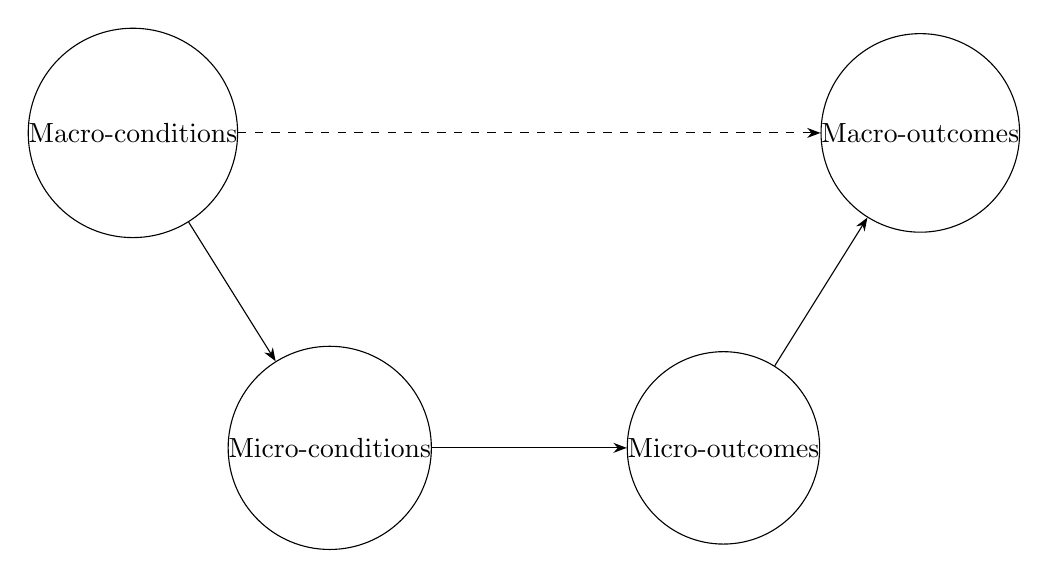
\begin{tikzpicture}
			\node (Macro-conditions) at (-5, 3) [place] {Macro-conditions};
			\node (Macro-outcomes)     at (5, 3) [place] {Macro-outcomes};
			\node (Micro-conditions)      at (-2.5,-1) [place] {Micro-conditions};
			\node (Micro-outcomes) at (2.5,-1) [place] {Micro-outcomes};
			\path[draw][-Stealth,dashed] (Macro-conditions) -- (Macro-outcomes);
			\path[draw][-Stealth] (Micro-conditions) -- (Micro-outcomes);
			\path[draw][-Stealth] (Macro-conditions) -- (Micro-conditions);
			\path[draw][-Stealth] (Micro-outcomes) -- (Macro-outcomes);
		\end{tikzpicture}
	\end{figure}
	
	This model serves as a foundational framework for understanding the interplay between individual-level actions and system-level outcomes. By outlining how micro-level processes, such as individual decisions or interactions, aggregate to influence macro-level structures, and how macro-level constraints feedback to shape individual behavior, the model highlights the reciprocal relationship between these levels of analysis. 
	
\end{itemize}

\subsection*{Research Significance}
Studying the micro-macro linkage is crucial for understanding complex social phenomena. It provides explanations for patterns such as group cohesion, social stratification, and network evolution. By bridging the gap between individual actions and systemic outcomes, this approach offers a multi-level analytical framework to explore the dynamic nature of social systems\cite{heider_attitudes_1946,scott_micromacro_2018}. 

\subsection*{Key Theories and Methods}
\begin{itemize}
	\item Structural Balance Theory: This theory investigates how micro-level triadic balance impacts macro-level group divisions. It provides a foundational model for understanding stability and change in social networks\cite{cartwright_structural_1956,heider_attitudes_1946}.
	\item Coleman’s Micro-Macro Model: Coleman’s framework elaborates on how individual decisions aggregate into macro-level structures and how these structures feedback to shape individual opportunities and motivations\cite{coleman_foundations_1990,raub_micro-macro_2011}.
	\item Empirical Network Analysis: Researchers use quantitative methods to measure and analyze the relationships between individual behaviors and network features, offering a data-driven approach to understanding micro-macro dynamics\cite{freeman_centrality_1978,borgatti_ucinet_2002}.
\end{itemize}
By integrating these theories and methods, the study of micro-macro linkages provides a comprehensive lens to examine how individual-level dynamics and systemic-level structures are intertwined, advancing our understanding of social networks and their role in broader social processes.

In the context of digital networks, the study of micro-macro linkages reveals how individual behaviors and platform-level dynamics interact to create systemic patterns. These interactions, mediated by the unique affordances of digital platforms, give rise to distinct phenomena such as virality, polarization, and algorithmic biases. This section explores the bottom-up and top-down mechanisms and their implications for social network research under digital context. 

Individual behaviors in digital networks, such as sharing, liking, or commenting, serve as the foundation for macro-level outcomes. These actions, when aggregated across vast user bases, create large-scale phenomena like viral trends, global movements, or misinformation cascades. For instance, hashtags like \#MeToo began as personal stories of sexual harassment and assault, but their rapid adoption transformed them into a global social movement\cite{manikonda_metoo_2018}. Similarly, the spread of fake news on platforms like Twitter exemplifies how individual users' retweets and shares contribute to the amplification and dissemination of misinformation, often at speeds exceeding factual information\cite{vosoughi_spread_2018}. 

A critical aspect of these bottom-up dynamics is the scalability of digital networks. Unlike traditional networks constrained by physical proximity or social connections, digital platforms allow individuals to reach global audiences instantly. This scalability amplifies weak ties' role, enabling the spread of novel information across previously disconnected communities\cite{granovetter_strength_1973}. Furthermore, features like trending algorithms and user-generated hashtags reinforce collective actions, enabling decentralized yet highly coordinated behavior across diverse social groups.

In digital networks, top-down forces are predominantly mediated by platform algorithms, which shape user behavior through personalization, content recommendations, and visibility filters. Algorithms determine what content users see, whom they interact with, and even how they engage with the platform. For example, YouTube's recommendation system has been found to sometimes promote content that contradicts scientific consensus, potentially leading users into misinformation filter bubbles\cite{tomlein_audit_2021}. Similarly, social media platforms like Facebook and Twitter use algorithms to curate news feeds, shaping the flow of information and influencing individual posting and sharing behavior. 

These algorithms introduce biases that significantly impact micro-macro linkages. For instance, filter bubbles and echo chambers emerge when algorithms reinforce homophilic connections by recommending content or users similar to existing preferences\cite{pariser_filter_2011}. As a result, users are exposed to increasingly narrow viewpoints, leading to polarization at the macro level. Additionally, algorithms can amplify the reach of influencers or controversial content, disproportionately affecting network structures and creating power imbalances in information dissemination\cite{lazer_science_2018}.

Research into digital networks often examines how algorithmic interventions mediate micro-macro linkages, leading to emergent phenomena such as echo chambers and online polarization. Studies have shown that social media platforms can facilitate the rapid spread of both accurate information and misinformation, impacting public opinion and behavior on a large scale\cite{chowdhury_understanding_2023}. Understanding these dynamics is crucial for addressing challenges like digital inequality and the spread of misinformation.

Online polarization highlights the interplay between individual behaviors and systemic dynamics in digital networks. Studies have shown that micro-level interactions, such as selectively engaging with partisan content, aggregate into polarized macro-level structures that fragment public discourse\cite{bakshy_exposure_2015}. These dynamics underscore the need for new theoretical frameworks that integrate algorithmic mediation into traditional micro-macro models.

The study of micro-macro linkages in digital networks necessitates a multidisciplinary approach, combining insights from sociology, computer science, and behavioral economics. It also calls for the development of new methodologies to analyze the complex interplay between individual behaviors, algorithmic systems, and emergent network structures. 

\section{Reflections}\label{Reflections}

This paper has sought to explore the multifaceted dynamics of digital social networks, from their theoretical foundations to their practical implications. By examining the interplay between micro-level interactions and macro-level structures, we have shed light on the unique challenges and opportunities presented by digital platforms. The bibliometric analysis and discussion of key academic questions offer a snapshot of the evolving intellectual landscape, underscoring the depth and breadth of scholarly engagement with these issues.

Yet, much remains to be understood. The rapid pace of technological development continually reshapes the ways in which individuals connect, interact, and organize, often outpacing our theoretical frameworks. Algorithmic mediation, for instance, is a field ripe for further exploration, particularly in understanding its long-term sociological consequences. Similarly, the role of digital networks in exacerbating or mitigating inequalities warrants sustained and critical inquiry.

Rather than offering definitive conclusions, this work aims to serve as a foundation for future investigations, inviting researchers to deepen their engagement with the questions posed here. By fostering interdisciplinary collaboration and leveraging innovative methodologies, the academic community can continue to advance our understanding of digital networks and their impact on society.

In this sense, the study of digital networks is not merely a scholarly endeavor but an ongoing dialogue—a collective effort to grapple with the complexities of a digitally mediated world. This paper represents one step in that journey, with the hope that it will inspire further exploration and debate.

\pagebreak
\appendix
\section{WoS Query}
\label{app:query}

The search strategy employed targeted research on social networks using the following query: 

{\ttfamily\NavyBlue
	TS=("social network*") AND \\
	TS=("digital network*" OR "online social network*" OR "virtual network*" OR \\
	"computer-mediated communication" OR "internet-based interaction*" OR \\    
	"social network theor*" OR "network dynamic*" OR "tie formation" OR \\
	"micro-macro linkage*" OR "relational dynamic*" OR \\
	"information flow" OR "digital inequality" OR "algorithm* intervention*" OR \\
	"structural position*" OR "network structure*" OR \\
	"information diffusion" OR "misinformation" OR "echo chamber*" OR \\
	"filter bubble*" OR "homophily" OR "brokerage") and Multidisciplinary Sciences or \\
	Sociology or Social Sciences Interdisciplinary or Social Sciences Mathematical \\
	Methods (Web of Science Categories) and Social Sciences Citation Index (SSCI) \\ 
	or Science Citation Index Expanded (SCI-EXPANDED) (Web of Science Index) and \\
	Multidisciplinary Sciences or Sociology or Social Sciences Interdisciplinary or \\
	Social Sciences Mathematical Methods or Mathematics Interdisciplinary \\
	Applications or Communication or Computer Science Interdisciplinary Applications \\
	(Web of Science Categories)
}

\section{CiteSpace Configuration}
\label{app:config}
{\ttfamily\NavyBlue
	\begin{verbatim}
			"NounPhraseWordsMax": 4,
			"Description": "Bibliometrics of Digital Social Networks",
			"MaximumGMLNodeLabelLength": 8,
			"FilterByIntrinsicCitations": true,
			"AuthorED": false,
			"MaxLinksToRetain": 2.5,
			"AuthorGP": false,
			"SaveMergedSliceFiles": false,
			"UseC3": true,
			"DimensionsEndpoint": "https://app.dimensions.ai/",
			"ExclusionList": true,
			"ExportMatrix": false,
			"minimumThresholdValue": 1,
			"AliasList": true,
			"PercentageNodesToLabel": 1,
			"BurstWeight": 0,
			"UseAuthorFullname": true,
			"ConceptTreeHome": "C:\\Users\\Amethystium\\.citespace",
			"LookBackTime": -1,
			"MaxLinksPerNode": 10,
			"NormalizeCitations": false,
			"ExportSpace": false,
			"NounPhraseWordsMin": 2,
			"GlobalCheck": false,
			"NodeDegreeWeighted": true,
			"JDIC": true,
			"ExportAbstract": false,
			"LinkWeightModificationRate": 1.0E-11
	\end{verbatim}
}



\bibliographystyle{apalike}
\bibliography{citation}
\end{sloppypar}
\end{document}

%\subsubsection*{Authors}
%
%\begin{table}[htbp]
%	\centering
%	\caption{\label{table:Table3}Author Record Count}
%	\begin{tabular}{lr}
	%		\toprule
	%		Authors & Record Count \\
	%		\midrule
	%		Christakis NA & 22 \\
	%		Fowler JH & 16 \\
	%		Butts CT & 12 \\
	%		Snijders TAB & 12 \\
	%		Lomi A & 10 \\
	%		Buskens V & 9 \\
	%		Flache A & 9 \\
	%		Kertész J & 9 \\
	%		Wang P & 9 \\
	%		Cebrian M & 8 \\
	%		Centola D & 8 \\
	%		Lehmann S & 8 \\
	%		Robins G & 8 \\
	%		Stadtfeld C & 8 \\
	%		Wang Y & 8 \\
	%		\bottomrule
	%	\end{tabular}
%\end{table}